\section{mr::base::vec3$<$ C, T $>$ Struct Template Reference}
\label{structmr_1_1base_1_1vec3}\index{mr::base::vec3@{mr::base::vec3}}
{\tt \#include $<$mr\-Vector.h$>$}

Inheritance diagram for mr::base::vec3$<$ C, T $>$::\begin{figure}[H]
\begin{center}
\leavevmode
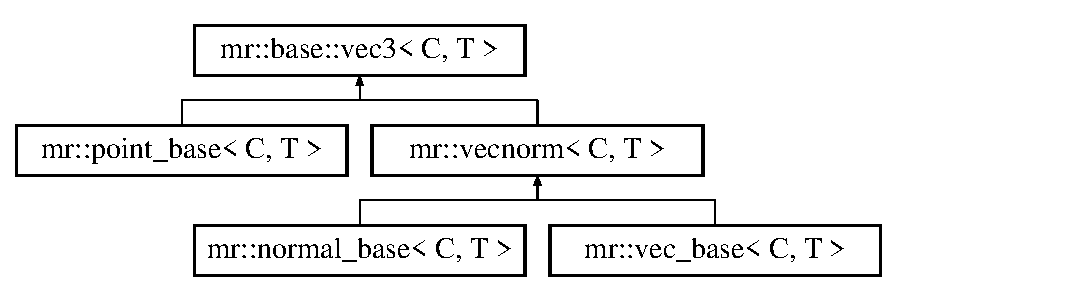
\includegraphics[height=3cm]{structmr_1_1base_1_1vec3}
\end{center}
\end{figure}
\subsection*{Public Types}
\begin{CompactItemize}
\item 
typedef {\bf vec3}$<$ C, T $>$ {\bf self}
\end{CompactItemize}
\subsection*{Public Member Functions}
\begin{CompactItemize}
\item 
const T {\bf Evaluate} (const unsigned short i) const 
\item 
{\bf operator mi\-Color} ()
\begin{CompactList}\small\item\em Conversion to mi\-Color. \item\end{CompactList}\item 
{\bf operator color} ()
\begin{CompactList}\small\item\em Conversion to color. \item\end{CompactList}\item 
{\bf vec3} ()
\begin{CompactList}\small\item\em Constructor that initializes x,y,z to 0. \item\end{CompactList}\item 
{\bf vec3} (const T xx, const T yy, const T zz)
\begin{CompactList}\small\item\em Constructor to initialize from three values. \item\end{CompactList}\item 
const bool {\bf is\-Equivalent} (const C \&b, const T tolerance=mi\-SCALAR\_\-EPSILON) const 
\item 
const {\bf self} \& {\bf mix} (const C \&b, const mi\-Scalar p)
\end{CompactItemize}
\begin{Indent}{\bf Accessors}\par
\begin{CompactItemize}
\item 
T \& {\bf operator[$\,$]} (const unsigned short i)
\begin{CompactList}\small\item\em Allow access to each element of vector for assignment. \item\end{CompactList}\item 
const T {\bf operator[$\,$]} (const unsigned short i) const 
\begin{CompactList}\small\item\em Allow access to each element of vector for reading. \item\end{CompactList}\item 
void {\bf set} (const unsigned short i, const T t)
\begin{CompactList}\small\item\em Allow assignment to an element of a vector. \item\end{CompactList}\item 
void {\bf set} (const T xx, const T yy, const T zz)
\begin{CompactList}\small\item\em Allow assignment to elements of a vector. \item\end{CompactList}\item 
T {\bf get} (const unsigned short i) const 
\begin{CompactList}\small\item\em Allow access to an element of vector for reading. \item\end{CompactList}\end{CompactItemize}
\end{Indent}
\begin{Indent}{\bf Assignment}\par
\begin{CompactItemize}
\item 
template$<$class X, class Y, class Oper$>$ const {\bf self} \& {\bf operator=} (const {\bf base::exp}$<$ X, Y, Oper $>$ \&e)
\begin{CompactList}\small\item\em Handle assignment when we deal with a chained operation. \item\end{CompactList}\item 
const {\bf self} \& {\bf operator=} (const {\bf self} \&b)
\begin{CompactList}\small\item\em Assignment of similar object. \item\end{CompactList}\item 
const {\bf self} \& {\bf operator=} (const C \&b)
\begin{CompactList}\small\item\em Assignemnt of base class object. \item\end{CompactList}\item 
const {\bf self} \& {\bf operator=} (const T b)
\begin{CompactList}\small\item\em Assignment of base type. \item\end{CompactList}\end{CompactItemize}
\end{Indent}
\begin{Indent}{\bf Equality}\par
\begin{CompactItemize}
\item 
template$<$class X, class Y, class Oper$>$ const bool {\bf operator==} (const {\bf base::exp}$<$ X, Y, Oper $>$ \&x) const 
\item 
const bool {\bf operator==} (const {\bf self} \&b) const 
\item 
const bool {\bf operator==} (const mi\-Vector \&b) const 
\item 
const bool {\bf operator==} (const T b) const 
\end{CompactItemize}
\end{Indent}
\begin{Indent}{\bf Inequality}\par
\begin{CompactItemize}
\item 
template$<$class X, class Y, class Oper$>$ const bool {\bf operator!=} (const {\bf base::exp}$<$ X, Y, Oper $>$ \&b) const 
\item 
const bool {\bf operator!=} (const {\bf self} \&b) const 
\item 
const bool {\bf operator!=} (const mi\-Vector \&b) const 
\item 
const bool {\bf operator!=} (const T b) const 
\end{CompactItemize}
\end{Indent}
\begin{Indent}{\bf REFERENCE OPERATORS (MODIFY IN PLACE)}\par
\begin{CompactItemize}
\item 
template$<$class X, class Y, class Oper$>$ const {\bf self} \& {\bf operator+=} (const {\bf base::exp}$<$ X, Y, Oper $>$ \&b)
\item 
const {\bf self} \& {\bf operator+=} (const T b)
\item 
const {\bf self} \& {\bf operator+=} (const C \&b)
\item 
template$<$class X, class Y, class Oper$>$ const {\bf self} \& {\bf operator-=} (const {\bf base::exp}$<$ X, Y, Oper $>$ \&b)
\item 
const {\bf self} \& {\bf operator-=} (const T b)
\item 
const {\bf self} \& {\bf operator-=} (const C \&b)
\item 
template$<$class X, class Y, class Oper$>$ const {\bf self} \& {\bf operator $\ast$=} (const {\bf base::exp}$<$ X, Y, Oper $>$ \&b)
\item 
const {\bf self} \& {\bf operator $\ast$=} (const T b)
\item 
const {\bf self} \& {\bf operator $\ast$=} (const C \&b)
\item 
template$<$class X, class Y, class Oper$>$ const {\bf self} \& {\bf operator/=} (const {\bf base::exp}$<$ X, Y, Oper $>$ \&b)
\item 
const {\bf self} \& {\bf operator/=} (const T b)
\item 
const {\bf self} \& {\bf operator/=} (const C \&b)
\end{CompactItemize}
\end{Indent}
\begin{Indent}{\bf Per channel comparisons}\par
\begin{CompactItemize}
\item 
{\bf self} {\bf less\-Than} (const C \&b)
\item 
{\bf self} {\bf less\-Than\-Equal} (const C \&b)
\item 
{\bf self} {\bf greater\-Than} (const C \&b)
\item 
{\bf self} {\bf greater\-Than\-Equal} (const C \&b)
\item 
const bool {\bf any} ()
\end{CompactItemize}
\end{Indent}
\begin{Indent}{\bf SWIZZLE OPERATORS}\par
\begin{CompactItemize}
\item 
const {\bf self} \& {\bf xyz} (const C \&t)
\item 
const {\bf self} \& {\bf xyz} (const {\bf self} \&t)
\item 
const {\bf self} \& {\bf xyz} () const 
\item 
const {\bf self} \& {\bf xyz} ()
\item 
{\bf self} {\bf xxx} () const 
\item 
{\bf self} {\bf yyy} () const 
\item 
{\bf self} {\bf zzz} () const 
\item 
{\bf self} {\bf zxy} () const 
\item 
{\bf self} {\bf yzx} () const 
\item 
{\bf self} {\bf zyx} () const 
\item 
{\bf self} {\bf yxz} () const 
\item 
{\bf self} {\bf yxx} () const 
\item 
{\bf self} {\bf zxx} () const 
\item 
{\bf self} {\bf xyx} () const 
\item 
{\bf self} {\bf xzx} () const 
\item 
{\bf self} {\bf xxy} () const 
\item 
{\bf self} {\bf xxz} () const 
\item 
{\bf self} {\bf xyy} () const 
\item 
{\bf self} {\bf zyy} () const 
\item 
{\bf self} {\bf yxy} () const 
\item 
{\bf self} {\bf yzy} () const 
\item 
{\bf self} {\bf yyx} () const 
\item 
{\bf self} {\bf yyz} () const 
\item 
{\bf self} {\bf yzz} () const 
\item 
{\bf self} {\bf xzz} () const 
\item 
{\bf self} {\bf zyz} () const 
\item 
{\bf self} {\bf zxz} () const 
\item 
{\bf self} {\bf zzy} () const 
\item 
{\bf self} {\bf zzx} () const 
\end{CompactItemize}
\end{Indent}
\subsubsection*{template$<$class C, class T$>$ struct mr::base::vec3$<$ C, T $>$}



\subsection{Member Typedef Documentation}
\index{mr::base::vec3@{mr::base::vec3}!self@{self}}
\index{self@{self}!mr::base::vec3@{mr::base::vec3}}
\subsubsection{\setlength{\rightskip}{0pt plus 5cm}template$<$class C, class T$>$ typedef {\bf vec3}$<$ C, T $>$ {\bf mr::base::vec3}$<$ C, T $>$::{\bf self}}\label{structmr_1_1base_1_1vec3_w0}




Reimplemented in {\bf mr::vecnorm$<$ C, T $>$} {\rm (p.\,\pageref{structmr_1_1vecnorm_w0})}, {\bf mr::vec\_\-base$<$ C, T $>$} {\rm (p.\,\pageref{structmr_1_1vec__base_w0})}, {\bf mr::normal\_\-base$<$ C, T $>$} {\rm (p.\,\pageref{structmr_1_1normal__base_w0})}, and {\bf mr::point\_\-base$<$ C, T $>$} {\rm (p.\,\pageref{structmr_1_1point__base_w0})}.

\subsection{Constructor \& Destructor Documentation}
\index{mr::base::vec3@{mr::base::vec3}!vec3@{vec3}}
\index{vec3@{vec3}!mr::base::vec3@{mr::base::vec3}}
\subsubsection{\setlength{\rightskip}{0pt plus 5cm}template$<$class C, class T$>$ {\bf mr::base::vec3}$<$ C, T $>$::{\bf vec3} ()\hspace{0.3cm}{\tt  [inline]}}\label{structmr_1_1base_1_1vec3_a3}


Constructor that initializes x,y,z to 0. 

\index{mr::base::vec3@{mr::base::vec3}!vec3@{vec3}}
\index{vec3@{vec3}!mr::base::vec3@{mr::base::vec3}}
\subsubsection{\setlength{\rightskip}{0pt plus 5cm}template$<$class C, class T$>$ {\bf mr::base::vec3}$<$ C, T $>$::{\bf vec3} (const T {\em xx}, const T {\em yy}, const T {\em zz})\hspace{0.3cm}{\tt  [inline]}}\label{structmr_1_1base_1_1vec3_a4}


Constructor to initialize from three values. 



\subsection{Member Function Documentation}
\index{mr::base::vec3@{mr::base::vec3}!any@{any}}
\index{any@{any}!mr::base::vec3@{mr::base::vec3}}
\subsubsection{\setlength{\rightskip}{0pt plus 5cm}template$<$class C, class T$>$ const bool {\bf mr::base::vec3}$<$ C, T $>$::any ()\hspace{0.3cm}{\tt  [inline]}}\label{structmr_1_1base_1_1vec3_z42_4}


\index{mr::base::vec3@{mr::base::vec3}!Evaluate@{Evaluate}}
\index{Evaluate@{Evaluate}!mr::base::vec3@{mr::base::vec3}}
\subsubsection{\setlength{\rightskip}{0pt plus 5cm}template$<$class C, class T$>$ const T {\bf mr::base::vec3}$<$ C, T $>$::Evaluate (const unsigned short {\em i}) const\hspace{0.3cm}{\tt  [inline]}}\label{structmr_1_1base_1_1vec3_a0}


\index{mr::base::vec3@{mr::base::vec3}!get@{get}}
\index{get@{get}!mr::base::vec3@{mr::base::vec3}}
\subsubsection{\setlength{\rightskip}{0pt plus 5cm}template$<$class C, class T$>$ T {\bf mr::base::vec3}$<$ C, T $>$::get (const unsigned short {\em i}) const\hspace{0.3cm}{\tt  [inline]}}\label{structmr_1_1base_1_1vec3_z35_4}


Allow access to an element of vector for reading. 

\index{mr::base::vec3@{mr::base::vec3}!greaterThan@{greaterThan}}
\index{greaterThan@{greaterThan}!mr::base::vec3@{mr::base::vec3}}
\subsubsection{\setlength{\rightskip}{0pt plus 5cm}template$<$class C, class T$>$ {\bf self} {\bf mr::base::vec3}$<$ C, T $>$::greater\-Than (const C \& {\em b})\hspace{0.3cm}{\tt  [inline]}}\label{structmr_1_1base_1_1vec3_z42_2}


\index{mr::base::vec3@{mr::base::vec3}!greaterThanEqual@{greaterThanEqual}}
\index{greaterThanEqual@{greaterThanEqual}!mr::base::vec3@{mr::base::vec3}}
\subsubsection{\setlength{\rightskip}{0pt plus 5cm}template$<$class C, class T$>$ {\bf self} {\bf mr::base::vec3}$<$ C, T $>$::greater\-Than\-Equal (const C \& {\em b})\hspace{0.3cm}{\tt  [inline]}}\label{structmr_1_1base_1_1vec3_z42_3}


\index{mr::base::vec3@{mr::base::vec3}!isEquivalent@{isEquivalent}}
\index{isEquivalent@{isEquivalent}!mr::base::vec3@{mr::base::vec3}}
\subsubsection{\setlength{\rightskip}{0pt plus 5cm}template$<$class C, class T$>$ const bool {\bf mr::base::vec3}$<$ C, T $>$::is\-Equivalent (const C \& {\em b}, const T {\em tolerance} = mi\-SCALAR\_\-EPSILON) const\hspace{0.3cm}{\tt  [inline]}}\label{structmr_1_1base_1_1vec3_a5}


\index{mr::base::vec3@{mr::base::vec3}!lessThan@{lessThan}}
\index{lessThan@{lessThan}!mr::base::vec3@{mr::base::vec3}}
\subsubsection{\setlength{\rightskip}{0pt plus 5cm}template$<$class C, class T$>$ {\bf self} {\bf mr::base::vec3}$<$ C, T $>$::less\-Than (const C \& {\em b})\hspace{0.3cm}{\tt  [inline]}}\label{structmr_1_1base_1_1vec3_z42_0}


\index{mr::base::vec3@{mr::base::vec3}!lessThanEqual@{lessThanEqual}}
\index{lessThanEqual@{lessThanEqual}!mr::base::vec3@{mr::base::vec3}}
\subsubsection{\setlength{\rightskip}{0pt plus 5cm}template$<$class C, class T$>$ {\bf self} {\bf mr::base::vec3}$<$ C, T $>$::less\-Than\-Equal (const C \& {\em b})\hspace{0.3cm}{\tt  [inline]}}\label{structmr_1_1base_1_1vec3_z42_1}


\index{mr::base::vec3@{mr::base::vec3}!mix@{mix}}
\index{mix@{mix}!mr::base::vec3@{mr::base::vec3}}
\subsubsection{\setlength{\rightskip}{0pt plus 5cm}template$<$class C, class T$>$ const {\bf self}\& {\bf mr::base::vec3}$<$ C, T $>$::mix (const C \& {\em b}, const mi\-Scalar {\em p})\hspace{0.3cm}{\tt  [inline]}}\label{structmr_1_1base_1_1vec3_a6}


\index{mr::base::vec3@{mr::base::vec3}!operator *=@{operator $\ast$=}}
\index{operator *=@{operator $\ast$=}!mr::base::vec3@{mr::base::vec3}}
\subsubsection{\setlength{\rightskip}{0pt plus 5cm}template$<$class C, class T$>$ const {\bf self}\& {\bf mr::base::vec3}$<$ C, T $>$::operator $\ast$= (const C \& {\em b})\hspace{0.3cm}{\tt  [inline]}}\label{structmr_1_1base_1_1vec3_z40_8}




Reimplemented in {\bf mr::vec\_\-base$<$ C, T $>$} {\rm (p.\,\pageref{structmr_1_1vec__base_z64_1})}, {\bf mr::normal\_\-base$<$ C, T $>$} {\rm (p.\,\pageref{structmr_1_1normal__base_z71_1})}, and {\bf mr::point\_\-base$<$ C, T $>$} {\rm (p.\,\pageref{structmr_1_1point__base_z78_1})}.\index{mr::base::vec3@{mr::base::vec3}!operator *=@{operator $\ast$=}}
\index{operator *=@{operator $\ast$=}!mr::base::vec3@{mr::base::vec3}}
\subsubsection{\setlength{\rightskip}{0pt plus 5cm}template$<$class C, class T$>$ const {\bf self}\& {\bf mr::base::vec3}$<$ C, T $>$::operator $\ast$= (const T {\em b})\hspace{0.3cm}{\tt  [inline]}}\label{structmr_1_1base_1_1vec3_z40_7}




Reimplemented in {\bf mr::vec\_\-base$<$ C, T $>$} {\rm (p.\,\pageref{structmr_1_1vec__base_z64_0})}, {\bf mr::normal\_\-base$<$ C, T $>$} {\rm (p.\,\pageref{structmr_1_1normal__base_z71_0})}, and {\bf mr::point\_\-base$<$ C, T $>$} {\rm (p.\,\pageref{structmr_1_1point__base_z78_0})}.\index{mr::base::vec3@{mr::base::vec3}!operator *=@{operator $\ast$=}}
\index{operator *=@{operator $\ast$=}!mr::base::vec3@{mr::base::vec3}}
\subsubsection{\setlength{\rightskip}{0pt plus 5cm}template$<$class C, class T$>$ template$<$class X, class Y, class Oper$>$ const {\bf self}\& {\bf mr::base::vec3}$<$ C, T $>$::operator $\ast$= (const {\bf base::exp}$<$ X, Y, Oper $>$ \& {\em b})\hspace{0.3cm}{\tt  [inline]}}\label{structmr_1_1base_1_1vec3_z40_6}


\index{mr::base::vec3@{mr::base::vec3}!operator color@{operator color}}
\index{operator color@{operator color}!mr::base::vec3@{mr::base::vec3}}
\subsubsection{\setlength{\rightskip}{0pt plus 5cm}template$<$class C, class T$>$ {\bf mr::base::vec3}$<$ C, T $>$::operator {\bf color} ()\hspace{0.3cm}{\tt  [inline]}}\label{structmr_1_1base_1_1vec3_a2}


Conversion to color. 

\index{mr::base::vec3@{mr::base::vec3}!operator miColor@{operator miColor}}
\index{operator miColor@{operator miColor}!mr::base::vec3@{mr::base::vec3}}
\subsubsection{\setlength{\rightskip}{0pt plus 5cm}template$<$class C, class T$>$ {\bf mr::base::vec3}$<$ C, T $>$::operator mi\-Color ()\hspace{0.3cm}{\tt  [inline]}}\label{structmr_1_1base_1_1vec3_a1}


Conversion to mi\-Color. 

\index{mr::base::vec3@{mr::base::vec3}!operator"!=@{operator"!=}}
\index{operator"!=@{operator"!=}!mr::base::vec3@{mr::base::vec3}}
\subsubsection{\setlength{\rightskip}{0pt plus 5cm}template$<$class C, class T$>$ const bool {\bf mr::base::vec3}$<$ C, T $>$::operator!= (const T {\em b}) const\hspace{0.3cm}{\tt  [inline]}}\label{structmr_1_1base_1_1vec3_z38_3}


\index{mr::base::vec3@{mr::base::vec3}!operator"!=@{operator"!=}}
\index{operator"!=@{operator"!=}!mr::base::vec3@{mr::base::vec3}}
\subsubsection{\setlength{\rightskip}{0pt plus 5cm}template$<$class C, class T$>$ const bool {\bf mr::base::vec3}$<$ C, T $>$::operator!= (const mi\-Vector \& {\em b}) const\hspace{0.3cm}{\tt  [inline]}}\label{structmr_1_1base_1_1vec3_z38_2}


\index{mr::base::vec3@{mr::base::vec3}!operator"!=@{operator"!=}}
\index{operator"!=@{operator"!=}!mr::base::vec3@{mr::base::vec3}}
\subsubsection{\setlength{\rightskip}{0pt plus 5cm}template$<$class C, class T$>$ const bool {\bf mr::base::vec3}$<$ C, T $>$::operator!= (const {\bf self} \& {\em b}) const\hspace{0.3cm}{\tt  [inline]}}\label{structmr_1_1base_1_1vec3_z38_1}


\index{mr::base::vec3@{mr::base::vec3}!operator"!=@{operator"!=}}
\index{operator"!=@{operator"!=}!mr::base::vec3@{mr::base::vec3}}
\subsubsection{\setlength{\rightskip}{0pt plus 5cm}template$<$class C, class T$>$ template$<$class X, class Y, class Oper$>$ const bool {\bf mr::base::vec3}$<$ C, T $>$::operator!= (const {\bf base::exp}$<$ X, Y, Oper $>$ \& {\em b}) const\hspace{0.3cm}{\tt  [inline]}}\label{structmr_1_1base_1_1vec3_z38_0}


\index{mr::base::vec3@{mr::base::vec3}!operator+=@{operator+=}}
\index{operator+=@{operator+=}!mr::base::vec3@{mr::base::vec3}}
\subsubsection{\setlength{\rightskip}{0pt plus 5cm}template$<$class C, class T$>$ const {\bf self}\& {\bf mr::base::vec3}$<$ C, T $>$::operator+= (const C \& {\em b})\hspace{0.3cm}{\tt  [inline]}}\label{structmr_1_1base_1_1vec3_z40_2}


\index{mr::base::vec3@{mr::base::vec3}!operator+=@{operator+=}}
\index{operator+=@{operator+=}!mr::base::vec3@{mr::base::vec3}}
\subsubsection{\setlength{\rightskip}{0pt plus 5cm}template$<$class C, class T$>$ const {\bf self}\& {\bf mr::base::vec3}$<$ C, T $>$::operator+= (const T {\em b})\hspace{0.3cm}{\tt  [inline]}}\label{structmr_1_1base_1_1vec3_z40_1}


\index{mr::base::vec3@{mr::base::vec3}!operator+=@{operator+=}}
\index{operator+=@{operator+=}!mr::base::vec3@{mr::base::vec3}}
\subsubsection{\setlength{\rightskip}{0pt plus 5cm}template$<$class C, class T$>$ template$<$class X, class Y, class Oper$>$ const {\bf self}\& {\bf mr::base::vec3}$<$ C, T $>$::operator+= (const {\bf base::exp}$<$ X, Y, Oper $>$ \& {\em b})\hspace{0.3cm}{\tt  [inline]}}\label{structmr_1_1base_1_1vec3_z40_0}


\index{mr::base::vec3@{mr::base::vec3}!operator-=@{operator-=}}
\index{operator-=@{operator-=}!mr::base::vec3@{mr::base::vec3}}
\subsubsection{\setlength{\rightskip}{0pt plus 5cm}template$<$class C, class T$>$ const {\bf self}\& {\bf mr::base::vec3}$<$ C, T $>$::operator-= (const C \& {\em b})\hspace{0.3cm}{\tt  [inline]}}\label{structmr_1_1base_1_1vec3_z40_5}


\index{mr::base::vec3@{mr::base::vec3}!operator-=@{operator-=}}
\index{operator-=@{operator-=}!mr::base::vec3@{mr::base::vec3}}
\subsubsection{\setlength{\rightskip}{0pt plus 5cm}template$<$class C, class T$>$ const {\bf self}\& {\bf mr::base::vec3}$<$ C, T $>$::operator-= (const T {\em b})\hspace{0.3cm}{\tt  [inline]}}\label{structmr_1_1base_1_1vec3_z40_4}


\index{mr::base::vec3@{mr::base::vec3}!operator-=@{operator-=}}
\index{operator-=@{operator-=}!mr::base::vec3@{mr::base::vec3}}
\subsubsection{\setlength{\rightskip}{0pt plus 5cm}template$<$class C, class T$>$ template$<$class X, class Y, class Oper$>$ const {\bf self}\& {\bf mr::base::vec3}$<$ C, T $>$::operator-= (const {\bf base::exp}$<$ X, Y, Oper $>$ \& {\em b})\hspace{0.3cm}{\tt  [inline]}}\label{structmr_1_1base_1_1vec3_z40_3}


\index{mr::base::vec3@{mr::base::vec3}!operator/=@{operator/=}}
\index{operator/=@{operator/=}!mr::base::vec3@{mr::base::vec3}}
\subsubsection{\setlength{\rightskip}{0pt plus 5cm}template$<$class C, class T$>$ const {\bf self}\& {\bf mr::base::vec3}$<$ C, T $>$::operator/= (const C \& {\em b})\hspace{0.3cm}{\tt  [inline]}}\label{structmr_1_1base_1_1vec3_z40_11}


\index{mr::base::vec3@{mr::base::vec3}!operator/=@{operator/=}}
\index{operator/=@{operator/=}!mr::base::vec3@{mr::base::vec3}}
\subsubsection{\setlength{\rightskip}{0pt plus 5cm}template$<$class C, class T$>$ const {\bf self}\& {\bf mr::base::vec3}$<$ C, T $>$::operator/= (const T {\em b})\hspace{0.3cm}{\tt  [inline]}}\label{structmr_1_1base_1_1vec3_z40_10}


\index{mr::base::vec3@{mr::base::vec3}!operator/=@{operator/=}}
\index{operator/=@{operator/=}!mr::base::vec3@{mr::base::vec3}}
\subsubsection{\setlength{\rightskip}{0pt plus 5cm}template$<$class C, class T$>$ template$<$class X, class Y, class Oper$>$ const {\bf self}\& {\bf mr::base::vec3}$<$ C, T $>$::operator/= (const {\bf base::exp}$<$ X, Y, Oper $>$ \& {\em b})\hspace{0.3cm}{\tt  [inline]}}\label{structmr_1_1base_1_1vec3_z40_9}


\index{mr::base::vec3@{mr::base::vec3}!operator=@{operator=}}
\index{operator=@{operator=}!mr::base::vec3@{mr::base::vec3}}
\subsubsection{\setlength{\rightskip}{0pt plus 5cm}template$<$class C, class T$>$ const {\bf self}\& {\bf mr::base::vec3}$<$ C, T $>$::operator= (const T {\em b})\hspace{0.3cm}{\tt  [inline]}}\label{structmr_1_1base_1_1vec3_z36_3}


Assignment of base type. 



Reimplemented in {\bf mr::vec\_\-base$<$ C, T $>$} {\rm (p.\,\pageref{structmr_1_1vec__base_z60_3})}, {\bf mr::normal\_\-base$<$ C, T $>$} {\rm (p.\,\pageref{structmr_1_1normal__base_z69_3})}, and {\bf mr::point\_\-base$<$ C, T $>$} {\rm (p.\,\pageref{structmr_1_1point__base_z77_3})}.\index{mr::base::vec3@{mr::base::vec3}!operator=@{operator=}}
\index{operator=@{operator=}!mr::base::vec3@{mr::base::vec3}}
\subsubsection{\setlength{\rightskip}{0pt plus 5cm}template$<$class C, class T$>$ const {\bf self}\& {\bf mr::base::vec3}$<$ C, T $>$::operator= (const C \& {\em b})\hspace{0.3cm}{\tt  [inline]}}\label{structmr_1_1base_1_1vec3_z36_2}


Assignemnt of base class object. 



Reimplemented in {\bf mr::vec\_\-base$<$ C, T $>$} {\rm (p.\,\pageref{structmr_1_1vec__base_z60_2})}, {\bf mr::normal\_\-base$<$ C, T $>$} {\rm (p.\,\pageref{structmr_1_1normal__base_z69_2})}, and {\bf mr::point\_\-base$<$ C, T $>$} {\rm (p.\,\pageref{structmr_1_1point__base_z77_2})}.\index{mr::base::vec3@{mr::base::vec3}!operator=@{operator=}}
\index{operator=@{operator=}!mr::base::vec3@{mr::base::vec3}}
\subsubsection{\setlength{\rightskip}{0pt plus 5cm}template$<$class C, class T$>$ const {\bf self}\& {\bf mr::base::vec3}$<$ C, T $>$::operator= (const {\bf self} \& {\em b})\hspace{0.3cm}{\tt  [inline]}}\label{structmr_1_1base_1_1vec3_z36_1}


Assignment of similar object. 



Reimplemented in {\bf mr::vec\_\-base$<$ C, T $>$} {\rm (p.\,\pageref{structmr_1_1vec__base_z60_1})}, {\bf mr::normal\_\-base$<$ C, T $>$} {\rm (p.\,\pageref{structmr_1_1normal__base_z69_1})}, and {\bf mr::point\_\-base$<$ C, T $>$} {\rm (p.\,\pageref{structmr_1_1point__base_z77_1})}.\index{mr::base::vec3@{mr::base::vec3}!operator=@{operator=}}
\index{operator=@{operator=}!mr::base::vec3@{mr::base::vec3}}
\subsubsection{\setlength{\rightskip}{0pt plus 5cm}template$<$class C, class T$>$ template$<$class X, class Y, class Oper$>$ const {\bf self}\& {\bf mr::base::vec3}$<$ C, T $>$::operator= (const {\bf base::exp}$<$ X, Y, Oper $>$ \& {\em e})\hspace{0.3cm}{\tt  [inline]}}\label{structmr_1_1base_1_1vec3_z36_0}


Handle assignment when we deal with a chained operation. 



Reimplemented in {\bf mr::vec\_\-base$<$ C, T $>$} {\rm (p.\,\pageref{structmr_1_1vec__base_z60_0})}, {\bf mr::normal\_\-base$<$ C, T $>$} {\rm (p.\,\pageref{structmr_1_1normal__base_z69_0})}, and {\bf mr::point\_\-base$<$ C, T $>$} {\rm (p.\,\pageref{structmr_1_1point__base_z77_0})}.\index{mr::base::vec3@{mr::base::vec3}!operator==@{operator==}}
\index{operator==@{operator==}!mr::base::vec3@{mr::base::vec3}}
\subsubsection{\setlength{\rightskip}{0pt plus 5cm}template$<$class C, class T$>$ const bool {\bf mr::base::vec3}$<$ C, T $>$::operator== (const T {\em b}) const\hspace{0.3cm}{\tt  [inline]}}\label{structmr_1_1base_1_1vec3_z37_3}


\index{mr::base::vec3@{mr::base::vec3}!operator==@{operator==}}
\index{operator==@{operator==}!mr::base::vec3@{mr::base::vec3}}
\subsubsection{\setlength{\rightskip}{0pt plus 5cm}template$<$class C, class T$>$ const bool {\bf mr::base::vec3}$<$ C, T $>$::operator== (const mi\-Vector \& {\em b}) const\hspace{0.3cm}{\tt  [inline]}}\label{structmr_1_1base_1_1vec3_z37_2}


\index{mr::base::vec3@{mr::base::vec3}!operator==@{operator==}}
\index{operator==@{operator==}!mr::base::vec3@{mr::base::vec3}}
\subsubsection{\setlength{\rightskip}{0pt plus 5cm}template$<$class C, class T$>$ const bool {\bf mr::base::vec3}$<$ C, T $>$::operator== (const {\bf self} \& {\em b}) const\hspace{0.3cm}{\tt  [inline]}}\label{structmr_1_1base_1_1vec3_z37_1}


\index{mr::base::vec3@{mr::base::vec3}!operator==@{operator==}}
\index{operator==@{operator==}!mr::base::vec3@{mr::base::vec3}}
\subsubsection{\setlength{\rightskip}{0pt plus 5cm}template$<$class C, class T$>$ template$<$class X, class Y, class Oper$>$ const bool {\bf mr::base::vec3}$<$ C, T $>$::operator== (const {\bf base::exp}$<$ X, Y, Oper $>$ \& {\em x}) const\hspace{0.3cm}{\tt  [inline]}}\label{structmr_1_1base_1_1vec3_z37_0}


\index{mr::base::vec3@{mr::base::vec3}!operator[]@{operator[]}}
\index{operator[]@{operator[]}!mr::base::vec3@{mr::base::vec3}}
\subsubsection{\setlength{\rightskip}{0pt plus 5cm}template$<$class C, class T$>$ const T {\bf mr::base::vec3}$<$ C, T $>$::operator[$\,$] (const unsigned short {\em i}) const\hspace{0.3cm}{\tt  [inline]}}\label{structmr_1_1base_1_1vec3_z35_1}


Allow access to each element of vector for reading. 

\index{mr::base::vec3@{mr::base::vec3}!operator[]@{operator[]}}
\index{operator[]@{operator[]}!mr::base::vec3@{mr::base::vec3}}
\subsubsection{\setlength{\rightskip}{0pt plus 5cm}template$<$class C, class T$>$ T\& {\bf mr::base::vec3}$<$ C, T $>$::operator[$\,$] (const unsigned short {\em i})\hspace{0.3cm}{\tt  [inline]}}\label{structmr_1_1base_1_1vec3_z35_0}


Allow access to each element of vector for assignment. 

\index{mr::base::vec3@{mr::base::vec3}!set@{set}}
\index{set@{set}!mr::base::vec3@{mr::base::vec3}}
\subsubsection{\setlength{\rightskip}{0pt plus 5cm}template$<$class C, class T$>$ void {\bf mr::base::vec3}$<$ C, T $>$::set (const T {\em xx}, const T {\em yy}, const T {\em zz})\hspace{0.3cm}{\tt  [inline]}}\label{structmr_1_1base_1_1vec3_z35_3}


Allow assignment to elements of a vector. 

\index{mr::base::vec3@{mr::base::vec3}!set@{set}}
\index{set@{set}!mr::base::vec3@{mr::base::vec3}}
\subsubsection{\setlength{\rightskip}{0pt plus 5cm}template$<$class C, class T$>$ void {\bf mr::base::vec3}$<$ C, T $>$::set (const unsigned short {\em i}, const T {\em t})\hspace{0.3cm}{\tt  [inline]}}\label{structmr_1_1base_1_1vec3_z35_2}


Allow assignment to an element of a vector. 

\index{mr::base::vec3@{mr::base::vec3}!xxx@{xxx}}
\index{xxx@{xxx}!mr::base::vec3@{mr::base::vec3}}
\subsubsection{\setlength{\rightskip}{0pt plus 5cm}template$<$class C, class T$>$ {\bf self} {\bf mr::base::vec3}$<$ C, T $>$::xxx () const\hspace{0.3cm}{\tt  [inline]}}\label{structmr_1_1base_1_1vec3_z44_4}


\index{mr::base::vec3@{mr::base::vec3}!xxy@{xxy}}
\index{xxy@{xxy}!mr::base::vec3@{mr::base::vec3}}
\subsubsection{\setlength{\rightskip}{0pt plus 5cm}template$<$class C, class T$>$ {\bf self} {\bf mr::base::vec3}$<$ C, T $>$::xxy () const\hspace{0.3cm}{\tt  [inline]}}\label{structmr_1_1base_1_1vec3_z44_15}


\index{mr::base::vec3@{mr::base::vec3}!xxz@{xxz}}
\index{xxz@{xxz}!mr::base::vec3@{mr::base::vec3}}
\subsubsection{\setlength{\rightskip}{0pt plus 5cm}template$<$class C, class T$>$ {\bf self} {\bf mr::base::vec3}$<$ C, T $>$::xxz () const\hspace{0.3cm}{\tt  [inline]}}\label{structmr_1_1base_1_1vec3_z44_16}


\index{mr::base::vec3@{mr::base::vec3}!xyx@{xyx}}
\index{xyx@{xyx}!mr::base::vec3@{mr::base::vec3}}
\subsubsection{\setlength{\rightskip}{0pt plus 5cm}template$<$class C, class T$>$ {\bf self} {\bf mr::base::vec3}$<$ C, T $>$::xyx () const\hspace{0.3cm}{\tt  [inline]}}\label{structmr_1_1base_1_1vec3_z44_13}


\index{mr::base::vec3@{mr::base::vec3}!xyy@{xyy}}
\index{xyy@{xyy}!mr::base::vec3@{mr::base::vec3}}
\subsubsection{\setlength{\rightskip}{0pt plus 5cm}template$<$class C, class T$>$ {\bf self} {\bf mr::base::vec3}$<$ C, T $>$::xyy () const\hspace{0.3cm}{\tt  [inline]}}\label{structmr_1_1base_1_1vec3_z44_17}


\index{mr::base::vec3@{mr::base::vec3}!xyz@{xyz}}
\index{xyz@{xyz}!mr::base::vec3@{mr::base::vec3}}
\subsubsection{\setlength{\rightskip}{0pt plus 5cm}template$<$class C, class T$>$ const {\bf self}\& {\bf mr::base::vec3}$<$ C, T $>$::xyz ()\hspace{0.3cm}{\tt  [inline]}}\label{structmr_1_1base_1_1vec3_z44_3}


\index{mr::base::vec3@{mr::base::vec3}!xyz@{xyz}}
\index{xyz@{xyz}!mr::base::vec3@{mr::base::vec3}}
\subsubsection{\setlength{\rightskip}{0pt plus 5cm}template$<$class C, class T$>$ const {\bf self}\& {\bf mr::base::vec3}$<$ C, T $>$::xyz () const\hspace{0.3cm}{\tt  [inline]}}\label{structmr_1_1base_1_1vec3_z44_2}


\index{mr::base::vec3@{mr::base::vec3}!xyz@{xyz}}
\index{xyz@{xyz}!mr::base::vec3@{mr::base::vec3}}
\subsubsection{\setlength{\rightskip}{0pt plus 5cm}template$<$class C, class T$>$ const {\bf self}\& {\bf mr::base::vec3}$<$ C, T $>$::xyz (const {\bf self} \& {\em t})\hspace{0.3cm}{\tt  [inline]}}\label{structmr_1_1base_1_1vec3_z44_1}


\index{mr::base::vec3@{mr::base::vec3}!xyz@{xyz}}
\index{xyz@{xyz}!mr::base::vec3@{mr::base::vec3}}
\subsubsection{\setlength{\rightskip}{0pt plus 5cm}template$<$class C, class T$>$ const {\bf self}\& {\bf mr::base::vec3}$<$ C, T $>$::xyz (const C \& {\em t})\hspace{0.3cm}{\tt  [inline]}}\label{structmr_1_1base_1_1vec3_z44_0}


\index{mr::base::vec3@{mr::base::vec3}!xzx@{xzx}}
\index{xzx@{xzx}!mr::base::vec3@{mr::base::vec3}}
\subsubsection{\setlength{\rightskip}{0pt plus 5cm}template$<$class C, class T$>$ {\bf self} {\bf mr::base::vec3}$<$ C, T $>$::xzx () const\hspace{0.3cm}{\tt  [inline]}}\label{structmr_1_1base_1_1vec3_z44_14}


\index{mr::base::vec3@{mr::base::vec3}!xzz@{xzz}}
\index{xzz@{xzz}!mr::base::vec3@{mr::base::vec3}}
\subsubsection{\setlength{\rightskip}{0pt plus 5cm}template$<$class C, class T$>$ {\bf self} {\bf mr::base::vec3}$<$ C, T $>$::xzz () const\hspace{0.3cm}{\tt  [inline]}}\label{structmr_1_1base_1_1vec3_z44_24}


\index{mr::base::vec3@{mr::base::vec3}!yxx@{yxx}}
\index{yxx@{yxx}!mr::base::vec3@{mr::base::vec3}}
\subsubsection{\setlength{\rightskip}{0pt plus 5cm}template$<$class C, class T$>$ {\bf self} {\bf mr::base::vec3}$<$ C, T $>$::yxx () const\hspace{0.3cm}{\tt  [inline]}}\label{structmr_1_1base_1_1vec3_z44_11}


\index{mr::base::vec3@{mr::base::vec3}!yxy@{yxy}}
\index{yxy@{yxy}!mr::base::vec3@{mr::base::vec3}}
\subsubsection{\setlength{\rightskip}{0pt plus 5cm}template$<$class C, class T$>$ {\bf self} {\bf mr::base::vec3}$<$ C, T $>$::yxy () const\hspace{0.3cm}{\tt  [inline]}}\label{structmr_1_1base_1_1vec3_z44_19}


\index{mr::base::vec3@{mr::base::vec3}!yxz@{yxz}}
\index{yxz@{yxz}!mr::base::vec3@{mr::base::vec3}}
\subsubsection{\setlength{\rightskip}{0pt plus 5cm}template$<$class C, class T$>$ {\bf self} {\bf mr::base::vec3}$<$ C, T $>$::yxz () const\hspace{0.3cm}{\tt  [inline]}}\label{structmr_1_1base_1_1vec3_z44_10}


\index{mr::base::vec3@{mr::base::vec3}!yyx@{yyx}}
\index{yyx@{yyx}!mr::base::vec3@{mr::base::vec3}}
\subsubsection{\setlength{\rightskip}{0pt plus 5cm}template$<$class C, class T$>$ {\bf self} {\bf mr::base::vec3}$<$ C, T $>$::yyx () const\hspace{0.3cm}{\tt  [inline]}}\label{structmr_1_1base_1_1vec3_z44_21}


\index{mr::base::vec3@{mr::base::vec3}!yyy@{yyy}}
\index{yyy@{yyy}!mr::base::vec3@{mr::base::vec3}}
\subsubsection{\setlength{\rightskip}{0pt plus 5cm}template$<$class C, class T$>$ {\bf self} {\bf mr::base::vec3}$<$ C, T $>$::yyy () const\hspace{0.3cm}{\tt  [inline]}}\label{structmr_1_1base_1_1vec3_z44_5}


\index{mr::base::vec3@{mr::base::vec3}!yyz@{yyz}}
\index{yyz@{yyz}!mr::base::vec3@{mr::base::vec3}}
\subsubsection{\setlength{\rightskip}{0pt plus 5cm}template$<$class C, class T$>$ {\bf self} {\bf mr::base::vec3}$<$ C, T $>$::yyz () const\hspace{0.3cm}{\tt  [inline]}}\label{structmr_1_1base_1_1vec3_z44_22}


\index{mr::base::vec3@{mr::base::vec3}!yzx@{yzx}}
\index{yzx@{yzx}!mr::base::vec3@{mr::base::vec3}}
\subsubsection{\setlength{\rightskip}{0pt plus 5cm}template$<$class C, class T$>$ {\bf self} {\bf mr::base::vec3}$<$ C, T $>$::yzx () const\hspace{0.3cm}{\tt  [inline]}}\label{structmr_1_1base_1_1vec3_z44_8}


\index{mr::base::vec3@{mr::base::vec3}!yzy@{yzy}}
\index{yzy@{yzy}!mr::base::vec3@{mr::base::vec3}}
\subsubsection{\setlength{\rightskip}{0pt plus 5cm}template$<$class C, class T$>$ {\bf self} {\bf mr::base::vec3}$<$ C, T $>$::yzy () const\hspace{0.3cm}{\tt  [inline]}}\label{structmr_1_1base_1_1vec3_z44_20}


\index{mr::base::vec3@{mr::base::vec3}!yzz@{yzz}}
\index{yzz@{yzz}!mr::base::vec3@{mr::base::vec3}}
\subsubsection{\setlength{\rightskip}{0pt plus 5cm}template$<$class C, class T$>$ {\bf self} {\bf mr::base::vec3}$<$ C, T $>$::yzz () const\hspace{0.3cm}{\tt  [inline]}}\label{structmr_1_1base_1_1vec3_z44_23}


\index{mr::base::vec3@{mr::base::vec3}!zxx@{zxx}}
\index{zxx@{zxx}!mr::base::vec3@{mr::base::vec3}}
\subsubsection{\setlength{\rightskip}{0pt plus 5cm}template$<$class C, class T$>$ {\bf self} {\bf mr::base::vec3}$<$ C, T $>$::zxx () const\hspace{0.3cm}{\tt  [inline]}}\label{structmr_1_1base_1_1vec3_z44_12}


\index{mr::base::vec3@{mr::base::vec3}!zxy@{zxy}}
\index{zxy@{zxy}!mr::base::vec3@{mr::base::vec3}}
\subsubsection{\setlength{\rightskip}{0pt plus 5cm}template$<$class C, class T$>$ {\bf self} {\bf mr::base::vec3}$<$ C, T $>$::zxy () const\hspace{0.3cm}{\tt  [inline]}}\label{structmr_1_1base_1_1vec3_z44_7}


\index{mr::base::vec3@{mr::base::vec3}!zxz@{zxz}}
\index{zxz@{zxz}!mr::base::vec3@{mr::base::vec3}}
\subsubsection{\setlength{\rightskip}{0pt plus 5cm}template$<$class C, class T$>$ {\bf self} {\bf mr::base::vec3}$<$ C, T $>$::zxz () const\hspace{0.3cm}{\tt  [inline]}}\label{structmr_1_1base_1_1vec3_z44_26}


\index{mr::base::vec3@{mr::base::vec3}!zyx@{zyx}}
\index{zyx@{zyx}!mr::base::vec3@{mr::base::vec3}}
\subsubsection{\setlength{\rightskip}{0pt plus 5cm}template$<$class C, class T$>$ {\bf self} {\bf mr::base::vec3}$<$ C, T $>$::zyx () const\hspace{0.3cm}{\tt  [inline]}}\label{structmr_1_1base_1_1vec3_z44_9}


\index{mr::base::vec3@{mr::base::vec3}!zyy@{zyy}}
\index{zyy@{zyy}!mr::base::vec3@{mr::base::vec3}}
\subsubsection{\setlength{\rightskip}{0pt plus 5cm}template$<$class C, class T$>$ {\bf self} {\bf mr::base::vec3}$<$ C, T $>$::zyy () const\hspace{0.3cm}{\tt  [inline]}}\label{structmr_1_1base_1_1vec3_z44_18}


\index{mr::base::vec3@{mr::base::vec3}!zyz@{zyz}}
\index{zyz@{zyz}!mr::base::vec3@{mr::base::vec3}}
\subsubsection{\setlength{\rightskip}{0pt plus 5cm}template$<$class C, class T$>$ {\bf self} {\bf mr::base::vec3}$<$ C, T $>$::zyz () const\hspace{0.3cm}{\tt  [inline]}}\label{structmr_1_1base_1_1vec3_z44_25}


\index{mr::base::vec3@{mr::base::vec3}!zzx@{zzx}}
\index{zzx@{zzx}!mr::base::vec3@{mr::base::vec3}}
\subsubsection{\setlength{\rightskip}{0pt plus 5cm}template$<$class C, class T$>$ {\bf self} {\bf mr::base::vec3}$<$ C, T $>$::zzx () const\hspace{0.3cm}{\tt  [inline]}}\label{structmr_1_1base_1_1vec3_z44_28}


\index{mr::base::vec3@{mr::base::vec3}!zzy@{zzy}}
\index{zzy@{zzy}!mr::base::vec3@{mr::base::vec3}}
\subsubsection{\setlength{\rightskip}{0pt plus 5cm}template$<$class C, class T$>$ {\bf self} {\bf mr::base::vec3}$<$ C, T $>$::zzy () const\hspace{0.3cm}{\tt  [inline]}}\label{structmr_1_1base_1_1vec3_z44_27}


\index{mr::base::vec3@{mr::base::vec3}!zzz@{zzz}}
\index{zzz@{zzz}!mr::base::vec3@{mr::base::vec3}}
\subsubsection{\setlength{\rightskip}{0pt plus 5cm}template$<$class C, class T$>$ {\bf self} {\bf mr::base::vec3}$<$ C, T $>$::zzz () const\hspace{0.3cm}{\tt  [inline]}}\label{structmr_1_1base_1_1vec3_z44_6}




The documentation for this struct was generated from the following file:\begin{CompactItemize}
\item 
{\bf mr\-Vector.h}\end{CompactItemize}
